\chapter{Implementation and Results}

This chapter documents the physics-informed neural network (PINN) built for the Lorenz-1960 system. It explains where the governing equations come from, traces each symbol into the source code, describes the network and its training, and reports the accuracy achieved. The entire pipeline is fundamentally built on PyTorch. The quantities that define the problem are imported from the baseline module rather than restated, so the equations exist in one place.

The method is built on stages and this chapter follows those stages in order.

\begin{table}[H]
\centering
\caption{How this chapter builds the method, stage by stage.}
\label{tab:roadmap}
\begin{spacing}{1.0}
\small
\begin{tabularx}{\textwidth}{|p{1.0cm}|>{\raggedright\arraybackslash}X|p{2.6cm}|}
\hline
\textbf{Stage} & \textbf{What it produces} & \textbf{Section} \\
\hline
1 & The problem: equations, coefficients $c$, initial state $u_0$, interval $[t_0, t_f]$ & \ref{sec:impl_equations} \\
\hline
2 & The baseline: reference trajectory $u^{\mathrm{ref}}$ & \ref{sec:impl_reference} \\
\hline
3 & The code map: modules and every symbol's definition site & \ref{sec:impl_software} \\
\hline
4 & The approximator: raw network $\mathcal{N}(t;\theta)$ & \ref{sec:impl_network} \\
\hline
5 & The trial solution $u_T(t)$, satisfying $u_T(t_0) = u_0$ by construction & \ref{sec:impl_ic} \\
\hline
6 & The residual $r(t)$: departure from the equations at one instant & \ref{sec:impl_residual} \\
\hline
7 & The collocation set $\{t_i\}_{i=1}^{N_c}$: where the residual is measured & \ref{sec:impl_collocation} \\
\hline
8 & The objective $\mathcal{L}(\theta)$ and the optimiser that minimises it & \ref{sec:impl_training} \\
\hline
9 & The measured error of the trained network against $u^{\mathrm{ref}}$ & \ref{sec:impl_results} \\
\hline
\end{tabularx}
\end{spacing}
\end{table}

\section{Governing Equations and Their Source}
\label{sec:impl_equations}

This section explains the problem and the equations on which the network is trained on. It also presents the coefficients of the Lorenz equations, the settings taken from the reference study, and the symbol mappings in the code. 


\subsection{The System and Its Coefficients}

The system consists of a Lorenz-1960 model in the form given by Matthews and Bihlo \cite{matthews2024pinnde}, Section 4.2, and reproduced as Equation~\ref{eq:lorenz1960} in Chapter~2. Parameters are general wavenumber $k$ and $l$,

\begin{equation}
\begin{aligned}
\frac{dx}{dt} &= kl\left(\frac{1}{k^2 + l^2} - \frac{1}{k^2}\right) yz, \\
\frac{dy}{dt} &= kl\left(\frac{1}{l^2} - \frac{1}{k^2 + l^2}\right) xz, \\
\frac{dz}{dt} &= \frac{kl}{2}\left(\frac{1}{k^2} - \frac{1}{l^2}\right) xy.
\end{aligned}
\label{eq:impl_lorenz_general}
\end{equation}

That reference states the system in Section 4.2 and gives code for it in Appendix A.2, and the two disagree. Section 4.2 is authoritative here. Appendix A.2 is not used.

The benchmark uses $k = 2$ and $l = 1$. Substitution gives three constants:

\begin{align}
c_x &= kl\left(\frac{1}{k^2 + l^2} - \frac{1}{k^2}\right) = 2\left(\frac{1}{5} - \frac{1}{4}\right) = -0.10, \label{eq:coeff_x}\\
c_y &= kl\left(\frac{1}{l^2} - \frac{1}{k^2 + l^2}\right) = 2\left(1 - \frac{1}{5}\right) = 1.60, \label{eq:coeff_y}\\
c_z &= \frac{kl}{2}\left(\frac{1}{k^2} - \frac{1}{l^2}\right) = 1\left(\frac{1}{4} - 1\right) = -0.75. \label{eq:coeff_z}
\end{align}

All three are exact in binary floating point. The reduced system solved by the network is therefore

\begin{equation}
\frac{dx}{dt} = -0.10\,yz, \qquad
\frac{dy}{dt} = 1.60\,xz, \qquad
\frac{dz}{dt} = -0.75\,xy.
\label{eq:impl_lorenz_reduced}
\end{equation}

The same source fixes the initial condition and the interval: $x(0) = 0.5$, $y(0) = 0.75$, $z(0) = 1$, and $t \in [0, 1]$. Writing $u = (x, y, z)$ and $u_0 = (0.5,\, 0.75,\, 1)$, the problem is the initial value problem $\dot{u} = f(u)$, $u(t_0) = u_0$, with $t_0 = 0$ and $t_f = 1$.

The coefficients are not hard-coded. The implementation calls \texttt{Lorenz-1960\_\allowbreak coefficients(k,\,l)} in the locked baseline, which evaluates Equations~\ref{eq:coeff_x}--\ref{eq:coeff_z} and returns $(-0.10,\, 1.60,\, -0.75)$. Changing $k$ or $l$ changes the equations without any edit to the network code.

\subsection{Adopted Settings and Notations}

Table~\ref{tab:adopted} separates what is taken from the reference study from what is chosen here. Section~\ref{sec:impl_comparison} returns to the differences.

\begin{table}[H]
\centering
\caption{Elements adopted from the reference study and elements chosen for this work.}
\label{tab:adopted}
\begin{spacing}{1.0}
\small
\begin{tabularx}{\textwidth}{|p{4.0cm}|>{\raggedright\arraybackslash}X|p{3.0cm}|}
\hline
\textbf{Element} & \textbf{Value} & \textbf{Source} \\
\hline
Equations, parameters, initial condition, interval & Equation~\ref{eq:impl_lorenz_general} with $k = 2$, $l = 1$; $u_0 = (0.5,\, 0.75,\, 1)$; $t \in [0, 1]$ & \cite{matthews2024pinnde}, Sec.~4.2 \\
\hline
Depth, width, activation & $4$ hidden layers of $60$ units, tanh & \cite{matthews2024pinnde}, Sec.~4.1 \\
\hline
Collocation and optimizer & $3000$ Latin hypercube points; Adam, $20{,}000$ iterations & \cite{matthews2024pinnde}, Sec.~4.1 \\
\hline
Initial-condition treatment & hard, by trial solution & this work, after \cite{lagaris1998ann} \\
\hline
Reference solver & DOP853 at $\text{rtol}=10^{-10}$ & this work \\
\hline
\end{tabularx}
\end{spacing}
\end{table}


\begin{table}[H]
\centering
\caption{Every symbol in this chapter and the code identifier that holds it.}
\label{tab:notation}
\begin{spacing}{1.0}
\small
\begin{tabularx}{\textwidth}{|p{2.9cm}|>{\raggedright\arraybackslash}X|p{4.6cm}|}
\hline
\textbf{Symbol} & \textbf{Meaning} & \textbf{Code identifier} \\
\hline
$t$ & Time, the single network input & \texttt{t} \\
\hline
$t_0 = 0$, $t_f = 1$ & Endpoints of the solution interval & \texttt{Config.t\_span} \\
\hline
$u = (x, y, z)$ & State vector & \texttt{u} \\
\hline
$u_0 = (0.5, 0.75, 1)$ & Initial state & \texttt{Config.initial\_state}, \texttt{PINN.u0} \\
\hline
$k = 2$, $l = 1$ & Wavenumbers & \texttt{Config.k}, \texttt{Config.l} \\
\hline
$c = (c_x, c_y, c_z)$ & Reduced coefficients & \texttt{lorenz1960\_coefficients} $\rightarrow$ \texttt{PINN.coeffs} \\
\hline
$f(u)$ & Right-hand side of the system & local \texttt{f} in \texttt{ode\_residual} \\
\hline
$\theta$ & Trainable parameters & \texttt{model.parameters()} \\
\hline
$\mathcal{N}(t;\theta)$ & Raw network output & \texttt{self.net(t)} \\
\hline
$L = 4$, $H = 60$ & Hidden layers, units per layer & \texttt{Config.depth}, \texttt{Config.width} \\
\hline
$g(t)$ & Ramp vanishing at $t_0$ & \texttt{g} in \texttt{PINN.forward} \\
\hline
$u_T(t)$ & Trial solution & return of \texttt{PINN.forward} \\
\hline
$r(t)$ & ODE residual & return of \texttt{residual} \\
\hline
$\{t_i\}_{i=1}^{N_c}$, $N_c = 3000$ & Collocation times & \texttt{grid}, \texttt{Config.n\_collocation} \\
\hline
$\mathcal{L}(\theta)$ & Training objective & \texttt{loss} in \texttt{train} \\
\hline
$\lambda_{\mathrm{IC}}$ & Soft-IC penalty weight, unused here & \texttt{Config.gamma} \\
\hline
$\{\tau_m\}_{m=1}^{M}$, $M = 1001$ & Evaluation times & reference grid, \texttt{n\_eval} \\
\hline
$u^{\mathrm{ref}}$ & DOP853 reference trajectory & \texttt{reference\_trajectory} \\
\hline
\end{tabularx}
\end{spacing}
\end{table}

The problem and the equations are now fully specified and broken down. But nothing can be trained until we have an independent solution to test the model against. Section~\ref{sec:impl_reference} shows the reference solution and how the baseline was created and verified. 

\section{Reference Solution}
\label{sec:impl_reference}

All the accuracy measurements are based on a numerical reference, which acts as the ground truth of the training. It's part of the locked baseline module \texttt{src/baseline/\allowbreak Lorenz-1960\_\allowbreak baseline.py}, which no code in this chapter modifies. Here, two independent methods are used. First, fourth order Runge-Kutta method with fixed step $h = 10^{-3}$ and second,  SciPy \texttt{solve\_ivp} with DOP853 at relative tolerance $10^{-10}$ and absolute tolerance $10^{-12}$. They both run over a  $1001$ uniformly distributed points. This grid is only used for baseline generation and for the model evaluation. They agree to $1.35 \times 10^{-11}$ RMSE, with a maximum difference of $6.06 \times 10^{-11}$. Two solvers of different order agreeing to eleven digits indicates that neither contains an implementation error.

All errors are measured with respect to the DOP853 trajectory. It is used only to score the trained network after optimizations. It provides no training signal and is not used anywhere in the loss.

The problem and the reference are both fixed now. Before the network and code base are explained, Section~\ref{sec:impl_software} shows where each of these concepts is defined in the code and which file reads it. 

\section{Software Architecture}
\label{sec:impl_software}

This section maps the problem of Section~\ref{sec:impl_equations} onto the code. The entire codebase breakdown and the configuration used in this research work. 

\subsection{The Module Map}

The implementation is the repository lorenz1960-pinn, available at \url{https://github.com/ihmorol/lorenz1960-pinn}. 
 Table~\ref{tab:modules} lists each Python file/module and the stages of Table~\ref{tab:roadmap} each module serves. 

\begin{table}[H]
\centering
\caption{Modules of the \texttt{fydp2} package and the sections they serve.}
\label{tab:modules}
\begin{spacing}{1.0}
\small
\begin{tabularx}{\textwidth}{|p{2.3cm}|>{\raggedright\arraybackslash}X|p{2.0cm}|}
\hline
\textbf{Module} & \textbf{Responsibility} & \textbf{Sections} \\
\hline
\texttt{config.py} & One fixed \texttt{Config} dataclass holding every setting. The only module that imports the locked baseline. & \ref{sec:impl_equations}, \ref{sec:impl_software} \\
\hline
\texttt{pinn.py} & Network, trial solution, ODE residual, and loss terms. & \ref{sec:impl_network}--\ref{sec:impl_residual} \\
\hline
\texttt{train.py} & Collocation grid, optimization loop, evaluation against the reference, results writer. & \ref{sec:impl_collocation}--\ref{sec:impl_results} \\
\hline
\texttt{history.py} & Per-iteration telemetry: loss components, gradient norms, learning rate, step size, reference error. & \ref{sec:impl_results} \\
\hline
\texttt{figures.py} & Figure suite and run report. Depends on NumPy and Matplotlib only, so figures rebuild without PyTorch. & \ref{sec:impl_results}, \ref{sec:impl_limitations} \\
\hline
\texttt{test\_pinn.py} & Automated checks on the initial condition, the residual, loss reduction, and figure generation. & \ref{sec:impl_training} \\
\hline
\end{tabularx}
\end{spacing}
\end{table}

The fields map onto the equations directly: \texttt{k} and \texttt{l} into Equation~\ref{eq:impl_lorenz_general}, \texttt{initial\_state} and \texttt{t\_span} into the trial solution of Equation~\ref{eq:trial}, and \texttt{n\_collocation} into the loss of Equation~\ref{eq:loss}. Because \texttt{coefficients} is a derived property rather than a stored constant, the equations follow $k$ and $l$ automatically.



\begin{lstlisting}[caption={The configuration object, abridged.}, label={lst:config}]
@dataclass(frozen=True)
class Config:
    k: float = 2.0                            # wavenumbers, Eq. 4.1
    l: float = 1.0
    initial_state: tuple = (0.5, 0.75, 1.0)   # u0
    t_span: tuple = (0.0, 1.0)                # [t0, tf]
    depth: int = 4                            # L, hidden layers
    width: int = 60                           # H, units per layer
    activation: str = "tanh"
    ic: str = "hard"                          # or "soft" (penalty)
    epochs: int = 20000
    lr_start, lr_end = 1e-3, 1e-4
    seed: int = 0
    n_collocation: int = 3000                 # N_c

    @property
    def coefficients(self) -> np.ndarray:     # -> (-0.10, 1.60, -0.75)
        return lorenz1960_coefficients(self.k, self.l)
\end{lstlisting}

\subsection{Configuration and Reproduction}

Listing~\ref{lst:config} shows the configuration object. One frozen data class carries the problem definition, the architecture, and the optimizer budget, so a run is fully described by a single value.

Table~\ref{tab:traceability} maps each element of the problem statement to the code that defines it and the code that uses it. No quantity has two definition sites.

\begin{table}[H]
\centering
\caption{Where each element of the problem definition is defined and used.}
\label{tab:traceability}
\begin{spacing}{1.0}
\small
\begin{tabularx}{\textwidth}{|p{2.6cm}|p{4.4cm}|>{\raggedright\arraybackslash}X|}
\hline
\textbf{Quantity} & \textbf{Defined at} & \textbf{Used by} \\
\hline
$k = 2$, $l = 1$ & \texttt{Config.k}, \texttt{Config.l} & \texttt{Config.coefficients} \\
\hline
$c_x, c_y, c_z$ & \texttt{lorenz1960\_coefficients} in the locked baseline & \texttt{ode\_residual}, via the \texttt{coeffs} buffer \\
\hline
$u_0$ & \texttt{Config.initial\_state} & \texttt{PINN.forward}; the reference solver \\
\hline
$t \in [0, 1]$ & \texttt{Config.t\_span} & \texttt{make\_grid}; the scaling function $g(t)$ \\
\hline
$f(u)$ & \texttt{ode\_residual} & \texttt{residual}, and through it the loss \\
\hline
Reference & \texttt{reference\_trajectory} & evaluation only \\
\hline
\end{tabularx}
\end{spacing}
\end{table}


\begin{lstlisting}[language=bash, numbers=none, caption={Reproducing the reported run from a clean checkout.}, label={lst:repro}]
pip install -r fydp2/requirements.txt
python run_pinn.py
\end{lstlisting}

Listing~\ref{lst:repro} reproduces the reported run: it trains the network, evaluates it against the reference, and writes the metric table and figures into \texttt{fydp2/results/}. The seed is fixed at $0$, so repeated runs give similar results on the same software versions. Because \texttt{history.py} stores telemetry beside the checkpoint, figures can be redrawn without retraining using \texttt{python run\_pinn.py -{}-figures}.

The settings of the workspace and the config object are now fixed. Now the first thing to build is the network itself, following Section~\ref{sec:impl_network} explains this stage. 

\section{Network Architecture}
\label{sec:impl_network}


The network maps scalar time $t$ to a three-component output (4 hidden layers of 60 with tanh activation). The tanh units are followed by a linear output layer with 3 units, giving $11{,}283$ trainable parameters. The raw output that the network produces is $\mathcal{N}(t;\theta)$, where the input time is $t$ and $\theta$ is the collection of all trainable parameters such as weights and biases. But the raw output isn't the final solution. The final solution is the Trial Solution approximation $u_T(t)=u_0+g(t)\mathcal{N}(t;\theta)$; this satisfies the initial condition by construction. Figure~\ref{fig:pinn_impl_arch} shows the full pipeline.

Figure~\ref{fig:pinn_impl_arch} shows the entire pipeline of the PINN architecture. Collocation times are shown on the top left. The raw output is then passed through the trial solution $u_T$ of Section~\ref{sec:impl_ic} to enforce the initial condition. The automatic differentiation provides $\dot{u}_T$.
Subtracts $f(u_T)$ from it is the residual of Section~\ref{sec:impl_residual}. Squaring and the loss is the average of that residual over the collocation point set.

\begin{figure}[H]
\centering
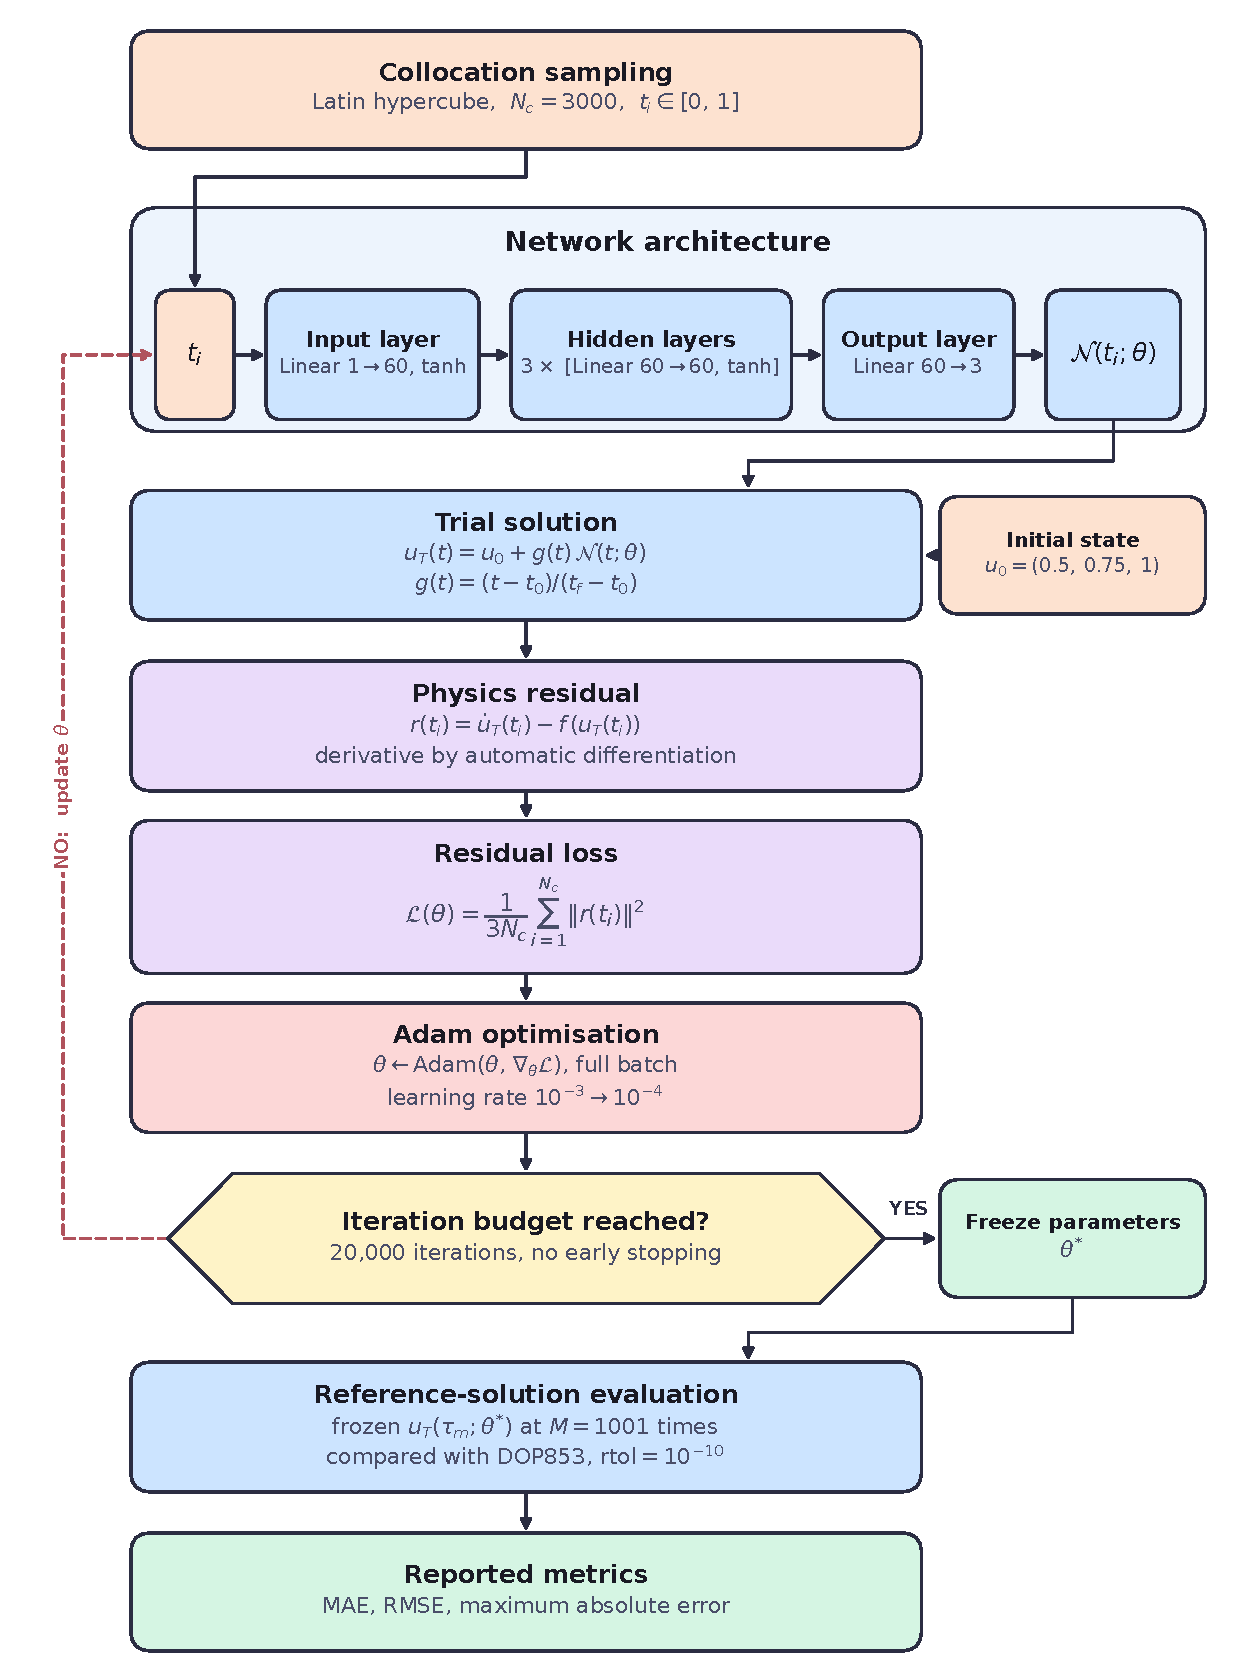
\includegraphics[width=\textwidth]{figures/fig_4_1_pinn_architecture.pdf}
\caption{Constructed pipeline of the Lorenz-1960 PINN.}
\label{fig:pinn_impl_arch}
\end{figure}

In this construction, the data term is empty, and the initial condition is imposed in construction through a trial solution. Weights use Xavier uniform initialization and biases start at zero.

\begin{lstlisting}[caption={Network construction. Depth, width, and activation come from \texttt{Config}, so the architecture is data rather than code.}, label={lst:mlp}]
act = _ACT[cfg.activation]                       # {"tanh": nn.Tanh, ...}
layers = [nn.Linear(1, cfg.width), act()]        # hidden layer 1
for _ in range(cfg.depth - 1):
    layers += [nn.Linear(cfg.width, cfg.width), act()]   # hidden layers 2..4
layers.append(nn.Linear(cfg.width, 3))           # linear output, (x, y, z)
self.net = nn.Sequential(*layers)

for m in self.net:
    if isinstance(m, nn.Linear):
        nn.init.xavier_uniform_(m.weight)
        nn.init.zeros_(m.bias)
\end{lstlisting}

 Listing~\ref{lst:mlp} builds the network, running the loop \texttt{depth - 1} times because the first hidden layer is constructed separately to take the single input feature.

 The initial condition is enforced using a trial solution and the following section explains how it was implemented. 

\section{Enforcing the Initial Condition}
\label{sec:impl_ic}

The initial condition is enforced structurally through a trial solution instead of learning, so training never spends computation on it. Building on the work of Lagaris et al.\ \cite{lagaris1998ann} and Babni et al.\ \cite{babni2025error}, the solution to the candidate is:

\begin{equation}
u_T(t) = u_0 + g(t)\,\mathcal{N}(t;\theta), \qquad g(t) = \frac{t - t_0}{t_f - t_0},
\label{eq:trial}
\end{equation}

where, $\mathcal{N}(t;\theta)$ represents the output of the raw network (Section~\ref{sec:impl_network}). Since  $t_0=0$ and $t_f=1$, the function becomes $g(t)=t$. Therefore, the equality $u_T(t_0) = u_0$ holds for any $\theta$.
Here the subscript $T$ in $u_T(t)$ means \emph{trial}.
The initial condition is enforced and satisfied to machine precision from the start, and cannot degrade during training. 

\begin{lstlisting}[caption={The forward pass, implementing Equation~\ref{eq:trial}.}, label={lst:forward}]
def forward(self, t: Tensor) -> Tensor:
    n = self.net(t)
    if self.ic == "hard":
        g = (t - self.t0) / (self.tf - self.t0)
        return self.u0 + g * n
    return n
\end{lstlisting}

A soft initial condition alternative is implemented through \texttt{Config(ic="soft")}. It follows the initial condition penalty term with coefficient $\lambda_{\mathrm{IC}}$, which needs to be tuned so that the two loss terms continue to be comparable, and it was added by Raissi et al.\ \cite{raissi2019pinn}. This hyperparameter is removed during the hard construction. All the results below refer to the hard construction.

The trial solution now enforces the net to satisfy the initial condition for every parameter. Now we need the model/net to agree on the Lorenz system equations ($\dot{u}_T$ agrees with
$f(u_T)$), Section~\ref{sec:impl_residual} breaks down the equation enforcement in the model through residuals at each collocation point.

\section{The Physics Residual}
\label{sec:impl_residual}

The residual is a measure of how far the candidate is from a solution of the equations:

\begin{equation}
r(t) = \frac{du_T}{dt} - f\big(u_T(t)\big),
\label{eq:residual}
\end{equation}

The residuals are zero when $u_T$ is exact. The derivative is derived from automatic differentiation, and which makes it the exact up to the floating-point precision. A finite-difference estimate would be followed by a truncation error near $10^{-6}$, which is similar to the desired accuracy, and would pollute the value of the quantity to be minimized.

Listing~\ref{lst:residual} is the only place where \texttt{ode\_residual} appears. It takes in the coefficient vector $c$ as an argument, which comes from \texttt{Config.coefficients}. The corresponding terms of the Equation~\ref{eq:impl_lorenz_reduced} are the products \texttt{y*z}, \texttt{x*z}, and \texttt{x*y}. 

\begin{lstlisting}[caption={The residual of Equation~\ref{eq:residual}, and the RHS it subtracts.}, label={lst:residual}]
def residual(model: PINN, t: Tensor) -> Tensor:
    u = model(t)                                  # trial solution, Eq. 4.6
    cols = [torch.autograd.grad(u[:, j].sum(), t,
                                create_graph=True)[0][:, 0]
            for j in range(u.shape[1])]           # d/dt of each component
    dudt = torch.stack(cols, dim=1)
    return ode_residual(u, dudt, model.coeffs)

def ode_residual(u: Tensor, dudt: Tensor, coeffs) -> Tensor:
    c = torch.as_tensor(coeffs, dtype=u.dtype, device=u.device).reshape(3)
    x, y, z = u[:, 0], u[:, 1], u[:, 2]
    f = torch.stack([c[0] * y * z,                # dx/dt = -0.10 y z
                     c[1] * x * z,                # dy/dt =  1.60 x z
                     c[2] * x * y], dim=1)        # dz/dt = -0.75 x y
    return dudt - f
\end{lstlisting}

In line 4, the argument \texttt{create\_graph=True} keeps $\dot{u}_T$ inside the auto-grad graph. Without keeping it, the derivative becomes constant. As a result, the optimizer can't back-propagate to reach $\theta$ through the residual. 
Equation~\ref{eq:residual} defines $r(t)$ at every $t$ in the interval. But training can only be possible in finitely many instants in the interval. Section~\ref{sec:impl_collocation} fixes this issue using collocation points. 

\section{Collocation Points}
\label{sec:impl_collocation}


The residual is enforced at $N_c = 3000$ instants $\{t_i\}_{i=1}^{N_c} \subset [t_0, t_f]$, randomly drawn and fixed in advance of training. The $N_c = 3000$ collocation points are used during the training and  $M=1001$ separate uniformly spaced points are used only to evaluate the model against the baseline. Both sets are in between $[0,1]$, so their different size are intentional. They are obtained from Latin hypercube sampling, which randomly selects a point in each of $N_c$ bins that divide the interval into equal-length subintervals. The drawback of this is that it causes clusters when using a uniform grid and a gap that is more than a bin wide when using an irregular grid; using Latin hypercube sampling solves it.


\begin{lstlisting}[caption={Generating the collocation grid. The sample comes from the unit interval then it was affinely mapped to the solution interval.}, label={lst:collocation}]
def make_grid(cfg: Config, device: torch.device) -> Tensor:
    t0, tf = cfg.t_span
    sample = qmc.LatinHypercube(d=1, seed=cfg.seed).random(cfg.n_collocation)
    t = t0 + (tf - t0) * sample                  # unit sample -> [t0, tf]
    return torch.as_tensor(t, dtype=torch.float32,
                           device=device).reshape(-1, 1)
\end{lstlisting}

The training is full batch, with all iterations evaluating the residuals, and no noise in the gradient arriving at any of the mini-batches.

Residuals in a finite set of instants are now available and Section~\ref{sec:impl_training} explains how we combine them into a single number that the training minimizes to learn. 

\section{Loss Function and Training Protocol}
\label{sec:impl_training}

The objective, or mean squared residual at the collocation points,

\begin{equation}
\mathcal{L}(\theta) = \frac{1}{3N_c} \sum_{i=1}^{N_c} \big\| r(t_i) \big\|^2 .
\label{eq:loss}
\end{equation}

The network is optimized with respect to these equations and if it is used alone, then the path it traces is determined by the residuals and an initial condition that was hard-wired into Equation~\ref{eq:trial}. The present implementation is different from the data-driven formulation of Chapter~2.

The number of optimization iterations with Adam is set to $20{,}000$, while the learning rate decays linearly from $10^{-3}$ to $10^{-4}$. The loop is listed in~\ref{lst:train}. The collocation grid is duplicated for every iteration because the tensor used to differentiate \texttt{requires\_grad\_} marks and the graph is discarded at the end of every back pass.

\begin{lstlisting}[caption={The training loop. \texttt{LambdaLR} on line 3 is linear interpolation started from the beginning and end learning rates across the entire budget.}, label={lst:train}]
adam = torch.optim.Adam(model.parameters(), lr=cfg.lr_start)
decay = cfg.lr_end / cfg.lr_start
sched = torch.optim.lr_scheduler.LambdaLR(
    adam, lambda e: 1.0 + (decay - 1.0) * min(e, cfg.epochs) / cfg.epochs)

for epoch in range(cfg.epochs):
    adam.zero_grad()
    res, ic = loss_terms(model, grid.clone().requires_grad_(True))
    loss = res + model.gamma * ic if cfg.ic == "soft" else res
    loss.backward()
    adam.step()
    sched.step()
\end{lstlisting}

The complete configuration is given in Table~\ref{tab:pinn_hyper}. An L-BFGS polishing stage is included in \texttt{train.py}. It also disables  \texttt{lbfgs\_iters = 0}, and therefore the results below are from Adam alone.

\begin{table}[H]
\centering
\caption{Training configuration for the reported run.}
\label{tab:pinn_hyper}
\begin{spacing}{1.0}
\small
\begin{tabular}{|l|l|l|l|}
\hline
\textbf{Setting} & \textbf{Value} & \textbf{Setting} & \textbf{Value} \\
\hline
Layers $\times$ width & $4 \times 60$ & Optimizer & Adam, full batch \\
\hline
Activation & tanh & Iterations & $20{,}000$ \\
\hline
Parameters & $11{,}263$ & Learning rate & $10^{-3}$ to $10^{-4}$, linear \\
\hline
Collocation points & $3000$, Latin hypercube & Precision & single (float32) \\
\hline
Initial condition & hard, Equation~\ref{eq:trial} & Random seed & $0$ \\
\hline
\end{tabular}
\end{spacing}
\end{table}

The architecture and the optimizer settings are taken from Section 4.1 of the reference study \cite{matthews2024pinnde}, which numerically solves the Euler rigid-body equations using PINN. Its Section 4.2, the source of the following solution to that system by a deep operator network, presumably done by the Lorenz-1960 equations. A multi-layer feed-forward network with four hidden layers of $40$ neurons each; soft initial conditions, $5000$ sampled initial conditions; and $75{,}000$ iterations. The following configuration is not found in any one of the experiments in that study, which is relevant to the interpretation of Section~\ref{sec:impl_comparison}.

Training is now fully specified and can be reproduced. Now we need to measure the trained network against the reference solution of Section~\ref{sec:impl_reference}.


\section{Model Evaluation}
\label{sec:impl_evaluation}

Training and evaluation are two vital phases of this research. There is no overlap between training and evaluation. The final iteration's parameters are frozen and stored. There were no early stops, and we selected the weights from the final iteration. The trained model is then evaluated against $M = 1001$ times $\{\tau_m\}$ of Section~\ref{sec:impl_reference}, here $\tau_m$ denote the $m$-th time of the evaluation grid. The model was not evaluated using the collocation points $\{t_i\}$ it was trained on.

\begin{lstlisting}[caption={The evaluation pass, abridged from \texttt{train.py}. The metrics of Table~\ref{tab:pinn_metrics} come from line 3.}, label={lst:evaluate}]
t, ref = reference_trajectory(cfg, n=1001)  # the evaluation grid
pred = predict(model, t)                    # frozen weights, no gradient
metrics = compute_error_metrics(ref, pred)  # MAE, RMSE, max |error| per state
metrics.to_csv(cfg.results_path / "metrics.csv", index=False)
\end{lstlisting}

\texttt{compute\_error\_metrics} uses the same three quantities for each state and for the correct one.
The sum of all the elements in Table~\ref{tab:pinn_metrics} is, known as the Euclidean norm of the error vector. The root mean squared error between the actual trajectory and the DOP853 trajectory, and the pointwise residual of Equation~\ref{eq:residual} over the interval. No evaluation time comes into the loss. No collocation time will be used in the metrics of Equation~\ref{eq:loss}. Section~\ref{sec:impl_results} reports the
numbers and the figures of training behavior and the solution.



\section{Results}
\label{sec:impl_results}

This section reports the performance of the trained network under the measures of Section~\ref{sec:impl_evaluation}. The error is calculated against the reference shown in Section~\ref{sec:impl_results_metrics}. And then is shown the solution, training behind it, and pointwise residuals are shown in detail with figures in Section~\ref{sec:impl_results_figures}. 

Over the time interval  $[0, 1]$ the trajectory moves from $(x, y, z) = (0.5, 0.75, 1.0)$ to $(0.412, 1.359, 0.631)$

\subsection{Error Metrics}
\label{sec:impl_results_metrics}

Table~\ref{tab:pinn_metrics} reports the error over the full $1001$-point grid. The combined row is the Euclidean magnitude of the three-component error vector, not an average.

\begin{table}[H]
\centering
\caption{Error of the trained PINN against the DOP853 reference over $1001$ points.}
\label{tab:pinn_metrics}
\begin{spacing}{1.0}
\small
\begin{tabular}{|l|l|l|l|}
\hline
\textbf{State} & \textbf{MAE} & \textbf{RMSE} & \textbf{Max. abs. error} \\
\hline
$x$ & $5.20 \times 10^{-6}$ & $5.77 \times 10^{-6}$ & $9.24 \times 10^{-6}$ \\
\hline
$y$ & $1.12 \times 10^{-5}$ & $1.36 \times 10^{-5}$ & $2.56 \times 10^{-5}$ \\
\hline
$z$ & $8.27 \times 10^{-6}$ & $9.04 \times 10^{-6}$ & $1.25 \times 10^{-5}$ \\
\hline
Combined $L_2$ & $1.66 \times 10^{-5}$ & $1.73 \times 10^{-5}$ & $2.60 \times 10^{-5}$ \\
\hline
\end{tabular}
\end{spacing}
\end{table}

Against states spanning $0.41$ to $1.36$, an error near $10^{-5}$ is close to five correct decimal. Without the network seeing any value of the solution, digits were retrieved. The largest errors fall in $y$, the state with the widest range and the largest coefficient.

\subsection{Solution and Training Behaviour}
\label{sec:impl_results_figures}

The trained solution is plotted against the reference in Figure~\ref{fig:solution}. All three states are smooth and monotone on $[0, 1]$: $x$ falls from $0.5$ to $0.412$, $y$ rises from $0.75$ to $1.359$, and $z$ falls from $1$ to $0.631$.

\begin{figure}[H]
\centering
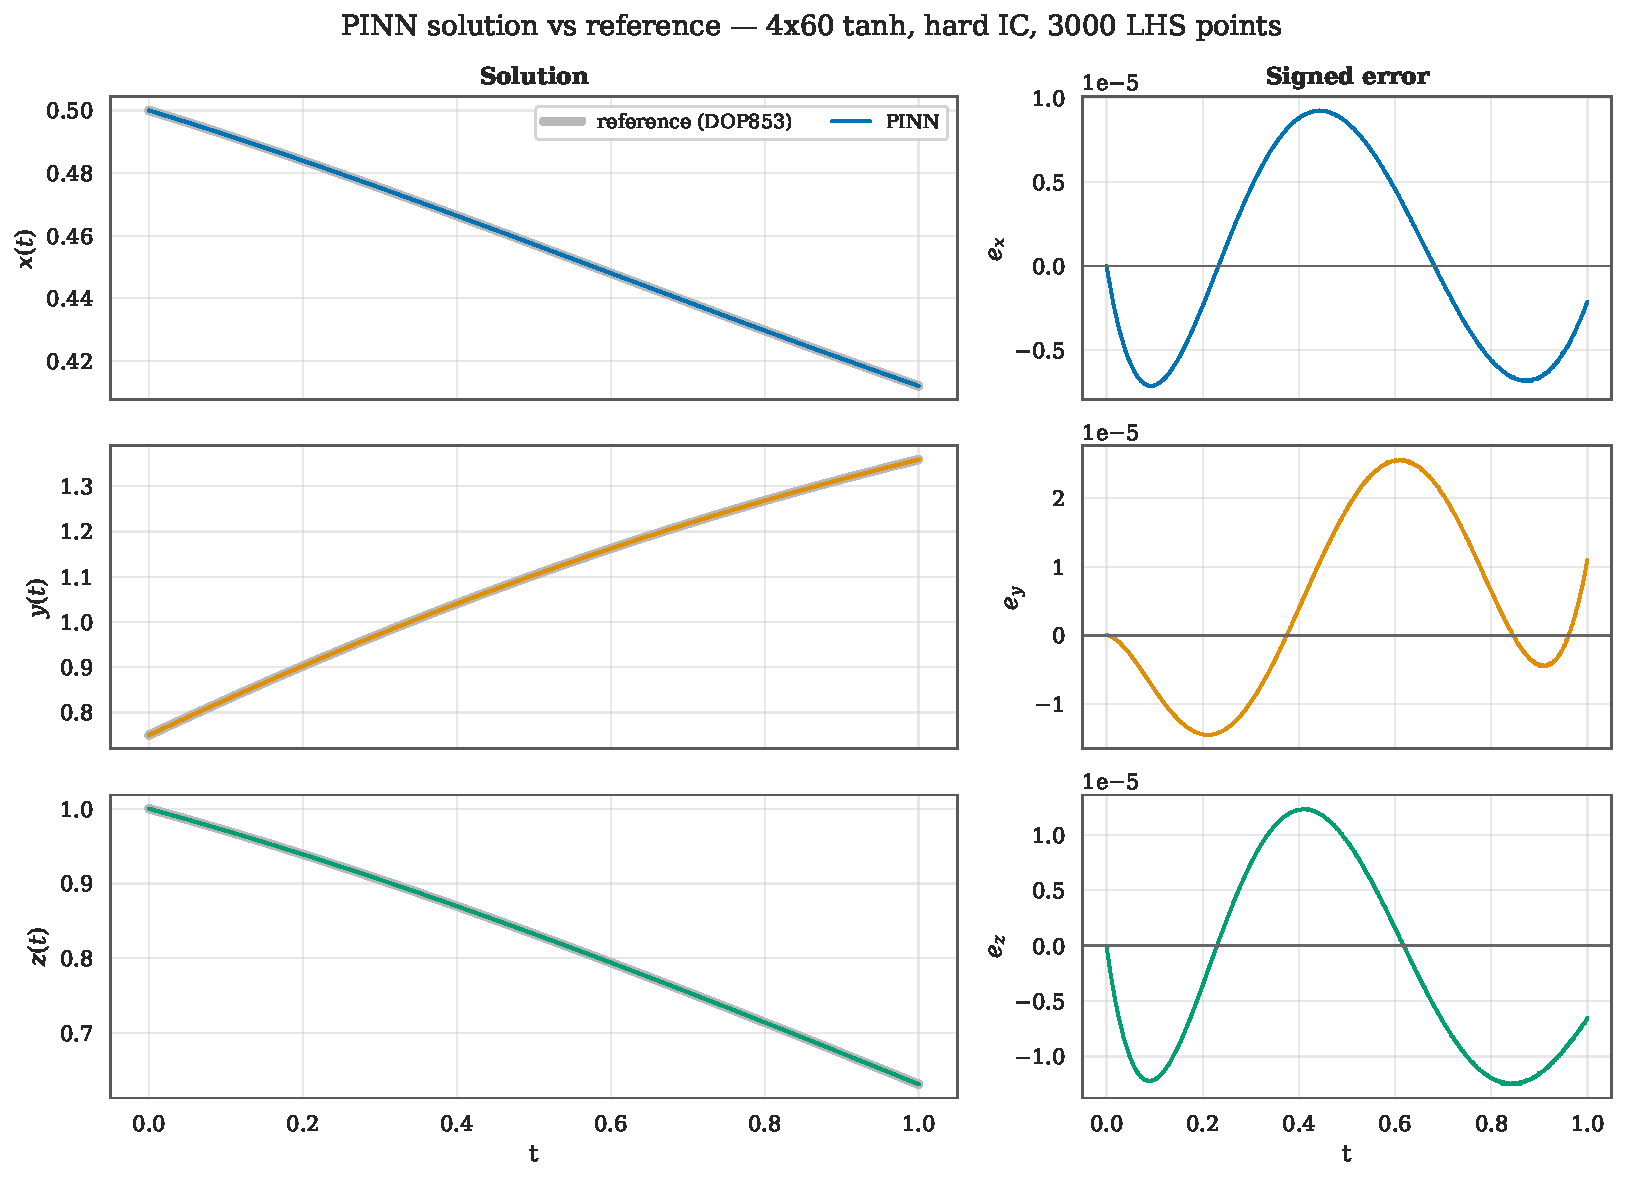
\includegraphics[width=0.85\textwidth]{figures/fig_4_2_solution_vs_reference.pdf}
\caption{PINN solution against the reference for each state, with the signed error beside each panel.}
\label{fig:solution}
\end{figure}

The training loss falls from $2.17 \times 10^{-1}$ to $6.82 \times 10^{-9}$ over the run, eight orders of magnitude. Also, there is no plateau or divergence.

\begin{figure}[H]
\centering
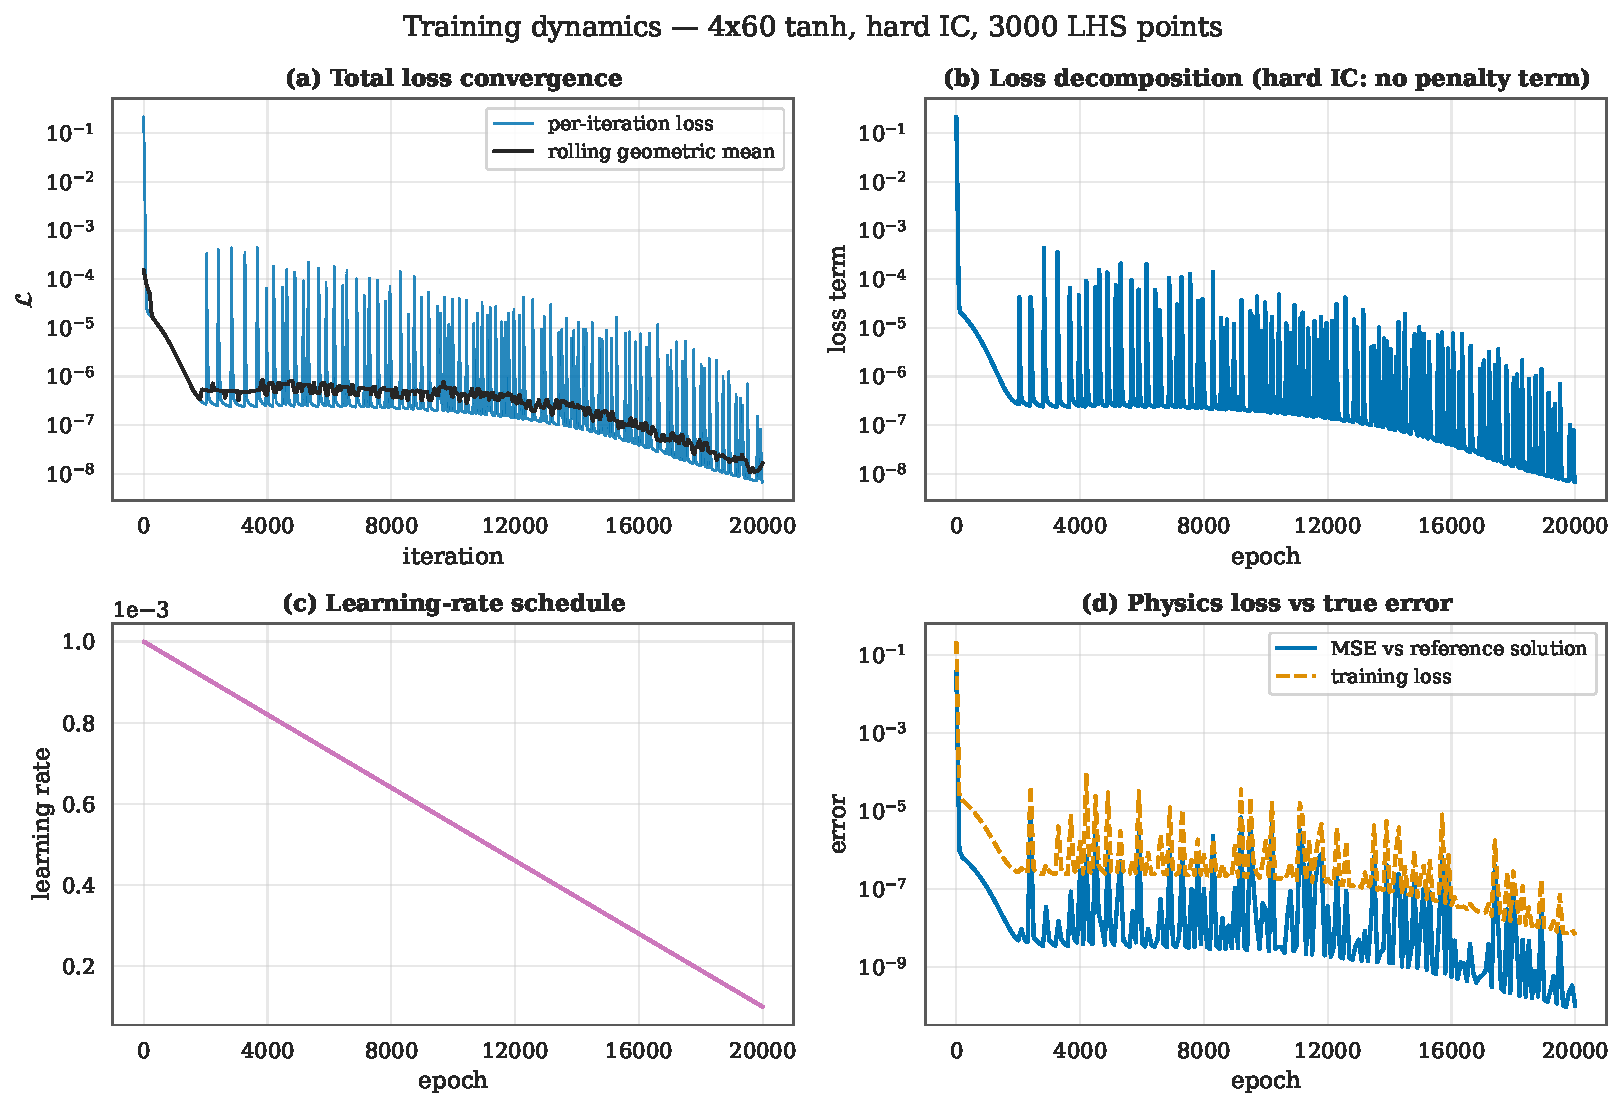
\includegraphics[width=0.80\textwidth]{figures/fig_4_3_training_dynamics.pdf}
\caption{Loss convergence, loss decomposition, learning-rate schedule, and reference error sampled every $100$ iterations.}
\label{fig:training}
\end{figure}

When a small average loss is obtained, the equations do not necessarily hold everywhere. Figure~\ref{fig:residual} shows the residual across the interval and confirms that they hold uniformly across the interval rather than in an average sense.

\begin{figure}[H]
\centering
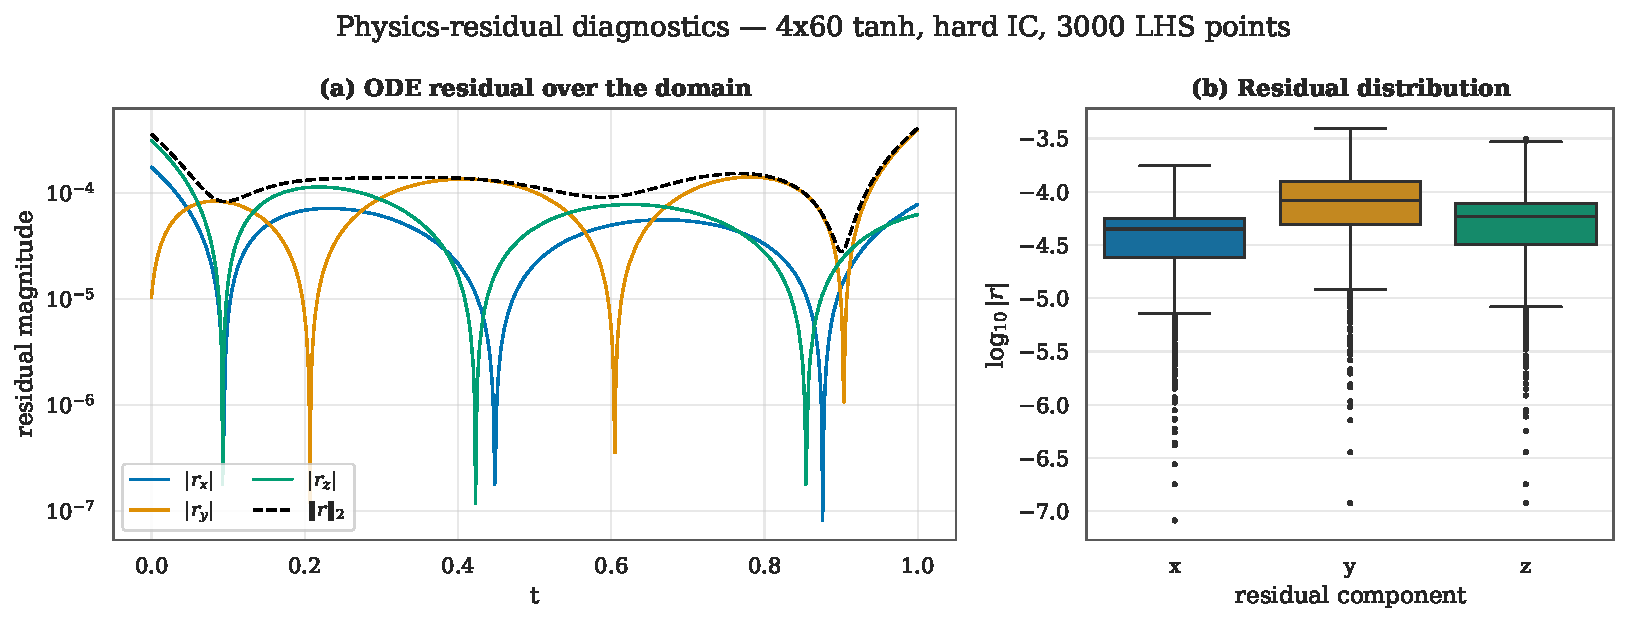
\includegraphics[width=0.80\textwidth]{figures/fig_4_4_physics_residual.pdf}
\caption{Magnitude of the ODE residual across the solution interval for the trained network.}
\label{fig:residual}
\end{figure}

\section{Comparison with the Reference Study}
\label{sec:impl_comparison}

Matthews and Bihlo \cite{matthews2024pinnde} present their Lorenz-1960 result as figures: the solution, the difference from a Runge-Kutta reference, and the training loss. They state that they use mean squared error as their metric, and they do not provide an error value table for this system. There is no direct numerical comparison to make, and no attempt is made to make such a comparison.  They have a difference plot that is consistent in order of magnitude with the data in Table~\ref{tab:pinn_metrics}, which is as much as a published figure supports.

Both designs are shown side by side in Table~\ref{tab:method_comparison}. The four settings vary, and any reading of the accuracy figures must account for all four. 

\begin{table}[H]
\centering
\caption{Method design compared with the reference study's Lorenz-1960 experiment.}
\label{tab:method_comparison}
\begin{spacing}{1.0}
\small
\begin{tabularx}{\textwidth}{|p{3.6cm}|>{\raggedright\arraybackslash}X|>{\raggedright\arraybackslash}X|}
\hline
\textbf{Aspect} & \textbf{\cite{matthews2024pinnde}, Sec.~4.2} & \textbf{This work} \\
\hline
Model class & Deep operator network & Physics-informed network \\
\hline
Layers $\times$ width & $4 \times 40$ & $4 \times 60$ \\
\hline
Initial condition & Soft, penalty in the loss & Hard, by trial solution \\
\hline
Initial conditions sampled & $5000$, over $[-2,2]^3$ & One, the benchmark value \\
\hline
Training iterations & $75{,}000$ & $20{,}000$ \\
\hline
What is learned & The solution operator $G(u_0)(t)$ & One trajectory $u(t)$ \\
\hline
Reported accuracy & Figures only & Table~\ref{tab:pinn_metrics} \\
\hline
\end{tabularx}
\end{spacing}
\end{table}

These two methods are addressing different questions. An operator network learns a mapping from initial conditions to solutions, a harder problem that explains both its larger budget and its soft constraints. The PINN here learns one trajectory, and the hard initial condition is available precisely because that trajectory is fixed in advance. The error table shown above appears to be the first published table of the numerical accuracy of a physics-informed solution of this system at these parameters.
